%!TEX root = paper.tex
\section{Results}\label{sec:results}

Below we present first results from studying the aggregate
traffic across the multiple \gls{lorawan} gateways operated
by volunteers in the \gls{oin} community.
The current results were generated with an Elasticsearch-based
tool that focuses on selected and aggregated metrics.
\todo[inline]{Hier fehlt noch ein Satz über Kibana. Wer betreibt diese Instanz? Basiert sie auch auf TTN, oder ist das was eigenes?}
Thus, we
cannot yet report on metrics such as message inter-arrival times,
collisions, or the number of distinct senders. However, we
to extend the tool for more in-depth analysis in the future.

Our dataset aggregates more than two million messages seen between
mid-April and mid-May 2018 across 13 gateways in an area of around
250 square kilometers in and around Vienna, Austria.
The gateways operate in diverse locations, ranging from window sills
and rooftops of private homes to tall office and industrial buildings
across the hilly region of Vienna. Accordingly, the area of reception
varies greatly; maximum reception distances exceed 60 kilometers for
some gateways, while others mainly work in their close neighborhood.
Gateways also differ in terms of time deployed, their the hardware, and
frequency channels supported by it. Similarly, senders differ
in terms of output power and channel use, amounts of data generated,
mobility, etc.
With this caveat, we turn to discussing our first results.

\begin{figure}
  \centering
  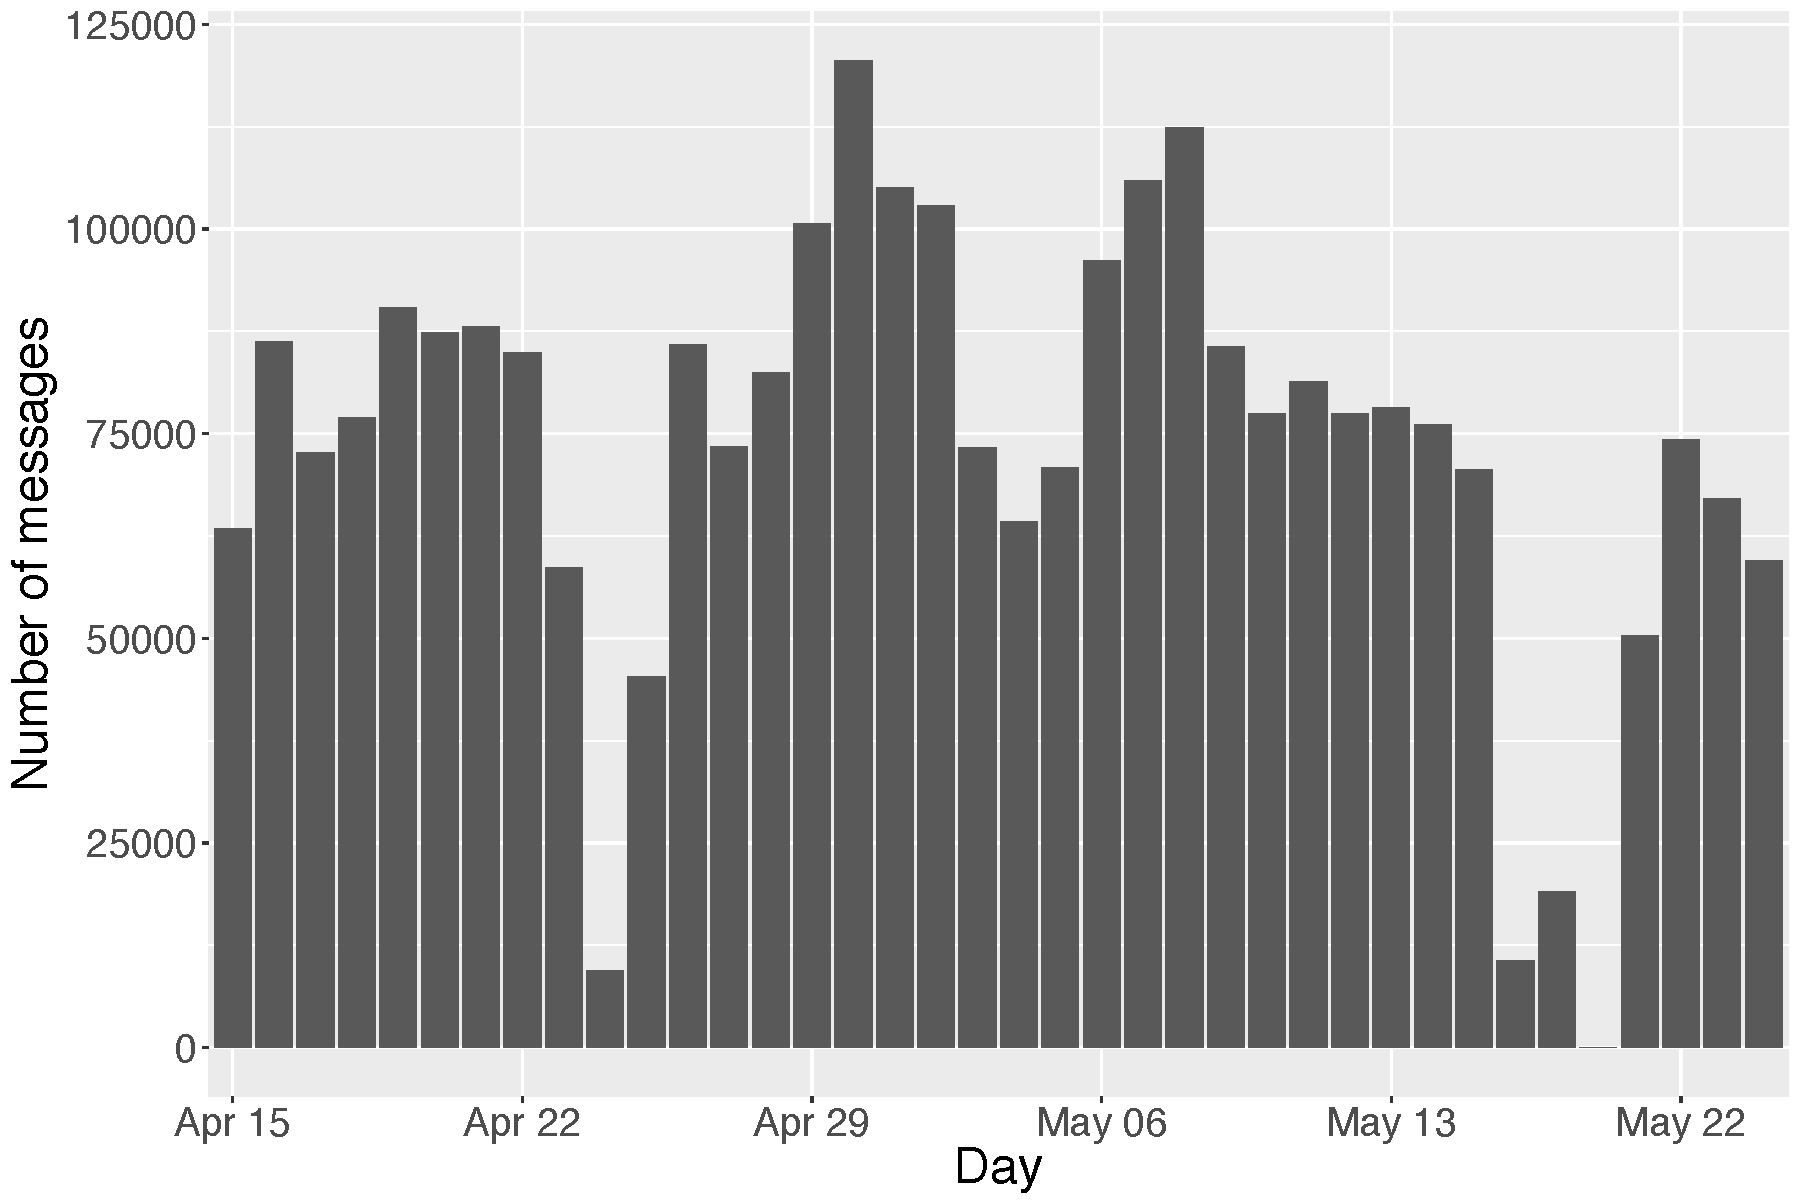
\includegraphics[width=\columnwidth]{figures/counts.pdf}
  \caption{Number of messages per day across all gateways (gray), and at the most active gateway (cyan).}
  \label{fig:counts}
\end{figure}

Figure~\ref{fig:counts} shows the number of messages per day for the
evaluated period. The system handles an average (and median) of over
73,000 messages per day, with peaks up to 120,000, corresponding to
per-second averages of 0.8 and 1.3. A closer look reveals peaks
of up to 3 messages per second. The most ``popular'' gateway
receives 25\% of all messages (highlighted in cyan in the figure);
the three runners-up account for
the next 25\% of messages received.
A few days of low (and even no) activity can be seen, but lacking
more detailed data at the moment, unfortunately we cannot reveal the
cause for these artifacts.

\begin{figure}
  \centering
  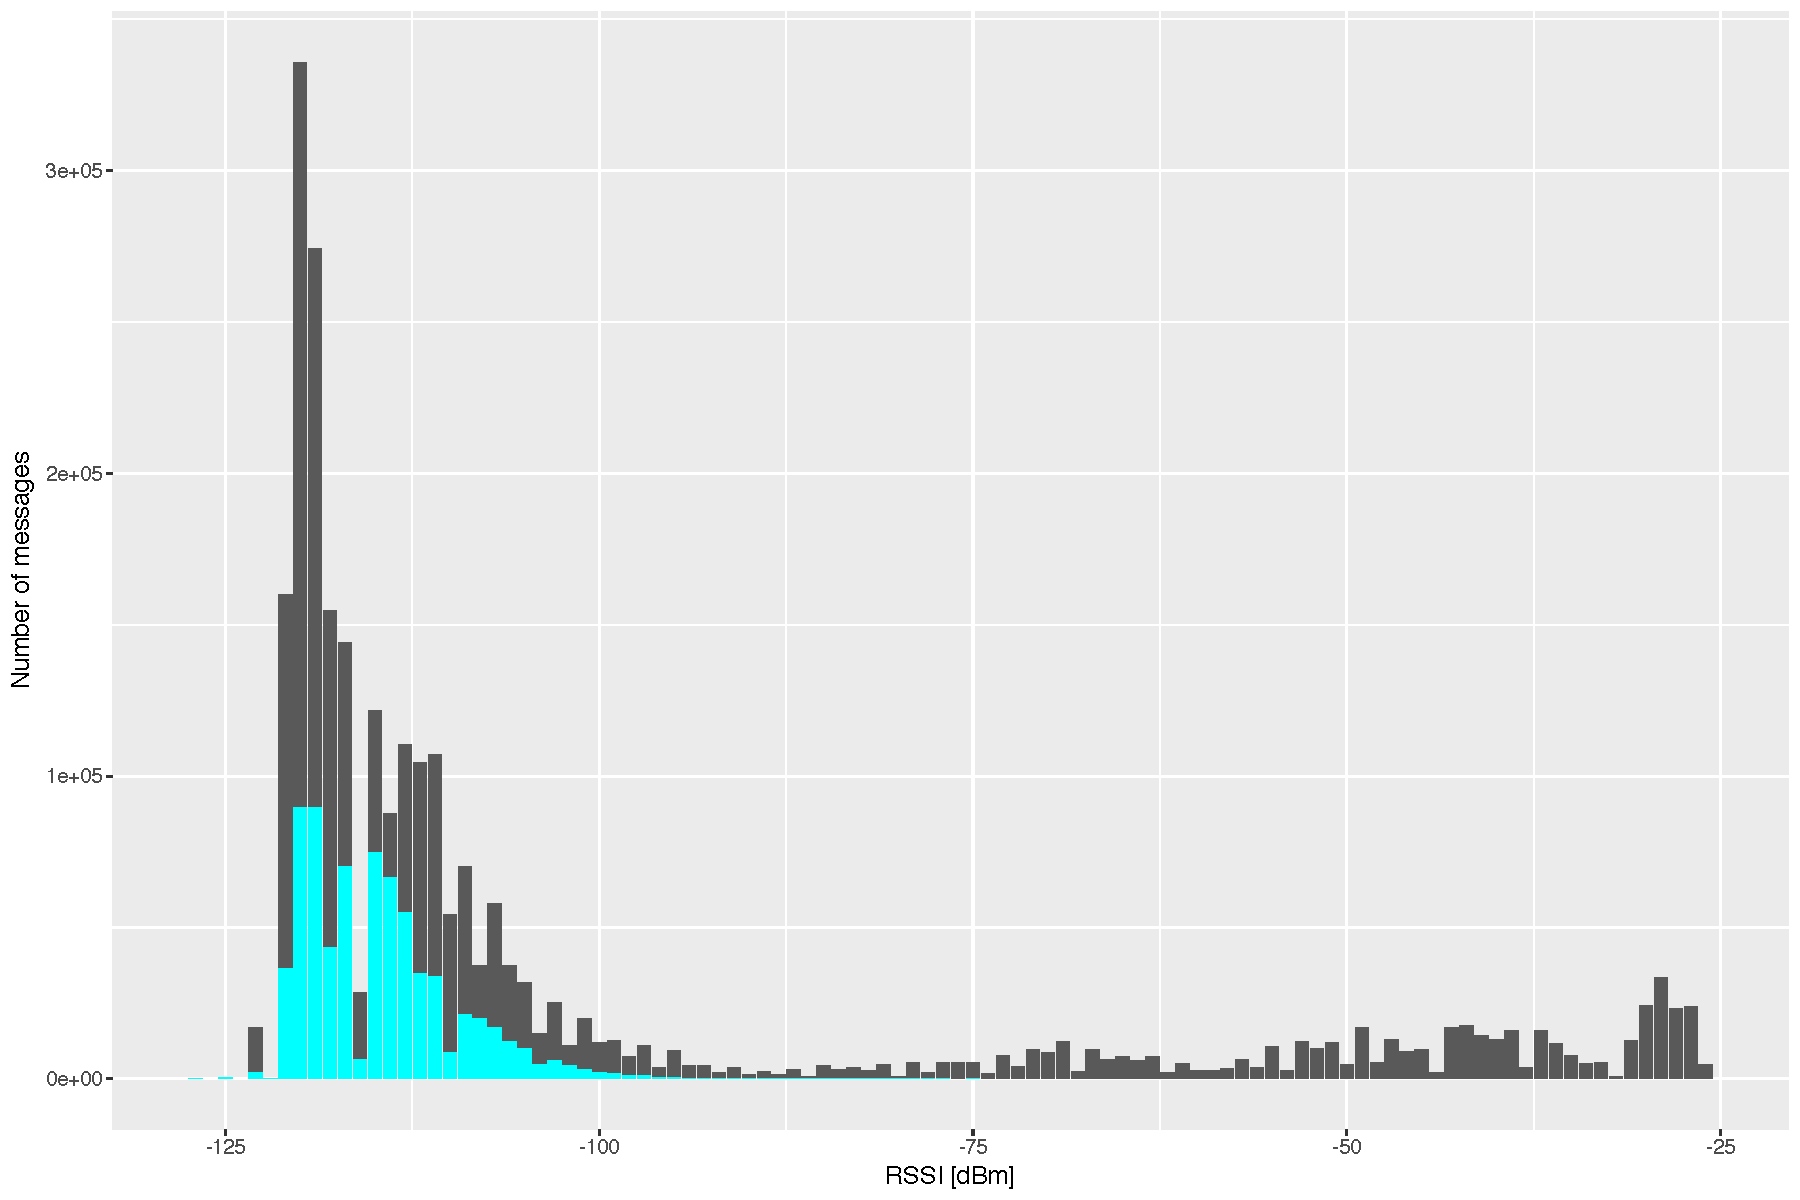
\includegraphics[width=\columnwidth]{figures/rssi.pdf}
  \caption{\acrshort{RSSI} for messages across all gateways (gray), and at the most active gateway (cyan).}
  \label{fig:rssi}
\end{figure}

Figure~\ref{fig:rssi} shows the \acrfull{RSSI} for messages across all
gateways (gray), and at the most active gateway (cyan).
Since the transmit power is unknown, the gateway hardware differs,
receive antenna gains are unknown, and the receivers are not calibrated,
the numbers should be interpreted with some caution.
Overall, the received power is of reasonable magnitude,
peaking around -120 dBm. The overall readings and those of
the most active gateway share roughly the same peaks and troughs
at low levels of receive power. We may speculate that the activity
and mobility of transmitters strongly shapes the figure: For instance,
an active and static sender will likely introduce a peak, whereas
mobile senders rather contribute to multiple bins. As noted before,
the topology of the landscape plays a role.

\begin{figure}
  \centering
  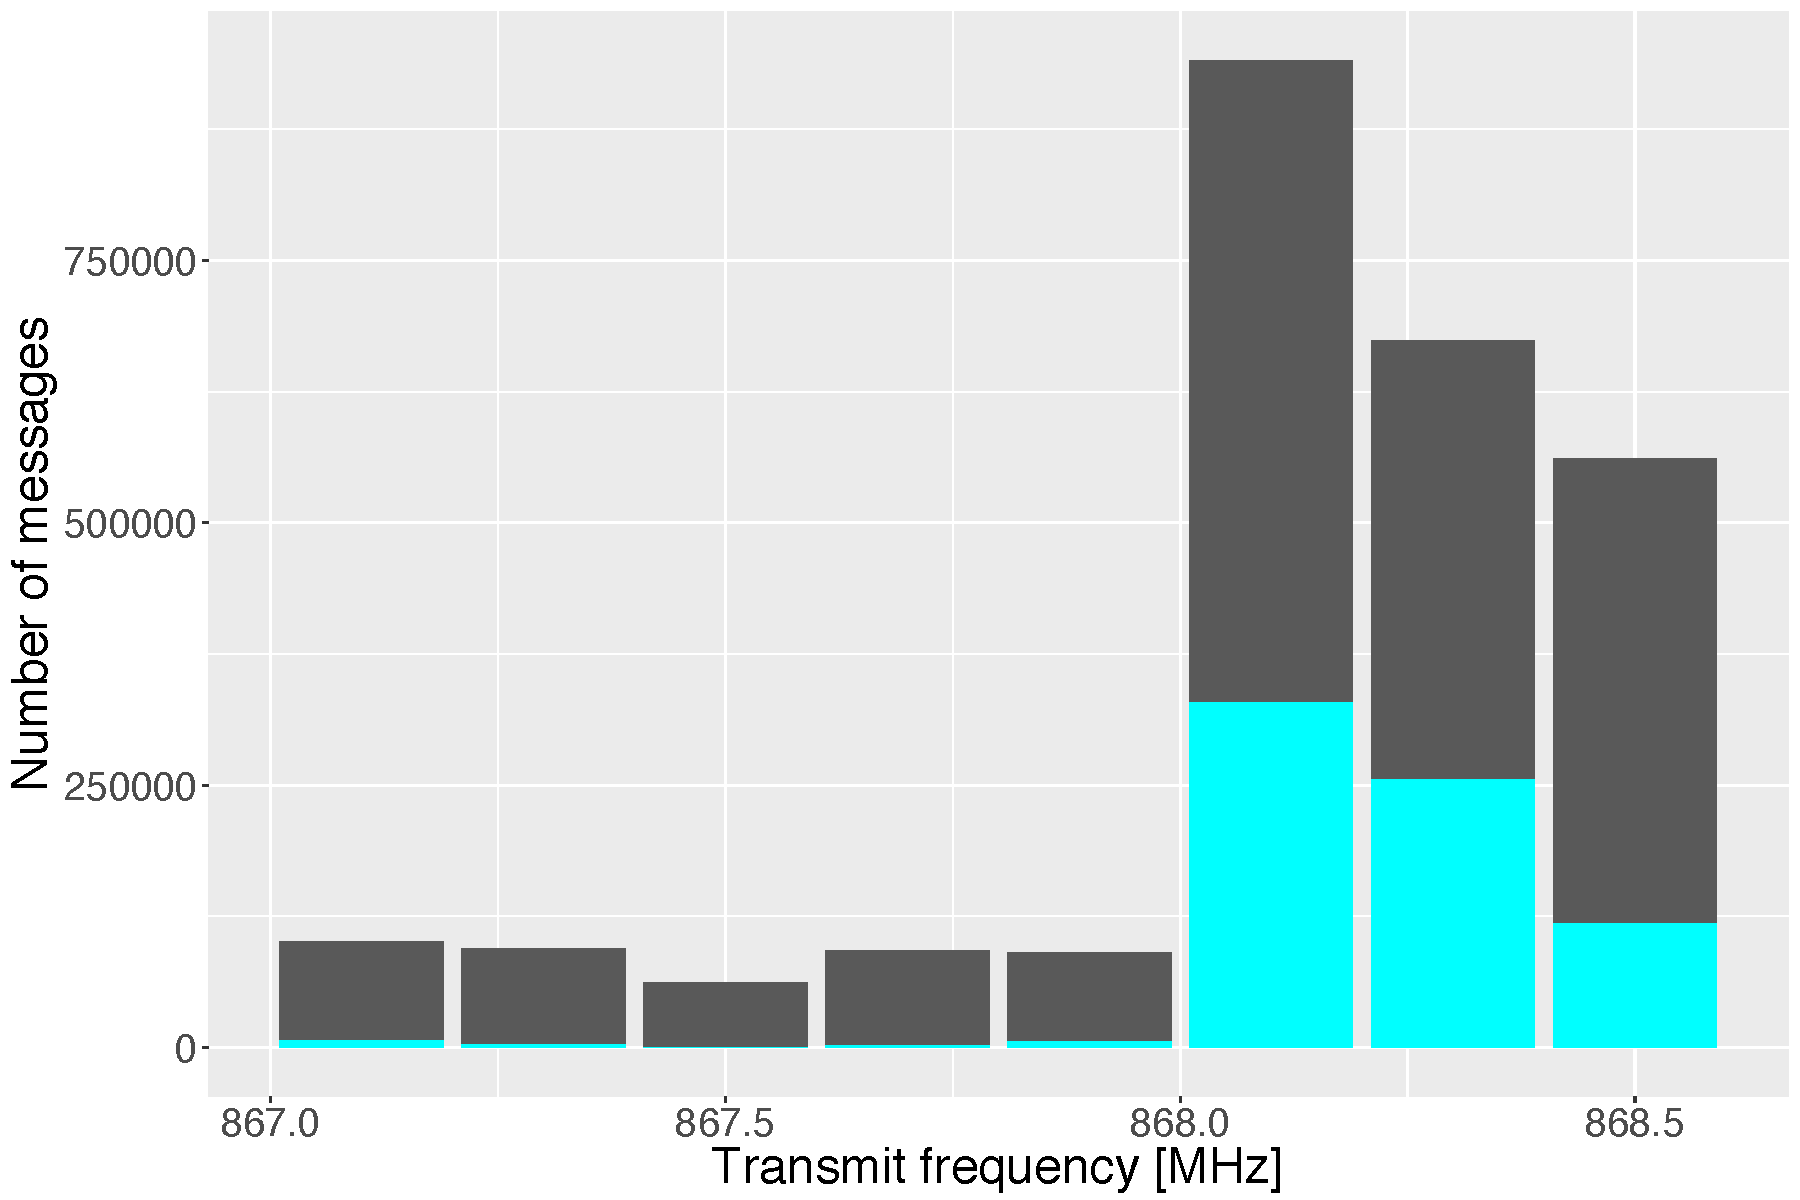
\includegraphics[width=\columnwidth]{figures/qrg.pdf}
  \caption{Transmission frequency for messages across all gateways (gray), and at the most active gateway (cyan).}
  \label{fig:qrg}
\end{figure}

Figure~\ref{fig:qrg} overviews the use of frequencies for transmissions
in the European \gls{SRD} band (863-870 MHz), as seen across all
gateways (gray) and at the most active gateway (cyan).
Evidently, transmissions on 868.1, .3 and .5 MHz dominate. The reason
is twofold: First, not all senders are able to use all channels.
Second, this is also true for gateways. The most active gateway,
while technically capable to receive on all eight channels, still
sees most of the messages on those three, indicating a sender-side
limitation. Other gateways do see uniform usage of channels.

\begin{figure}
  \centering
  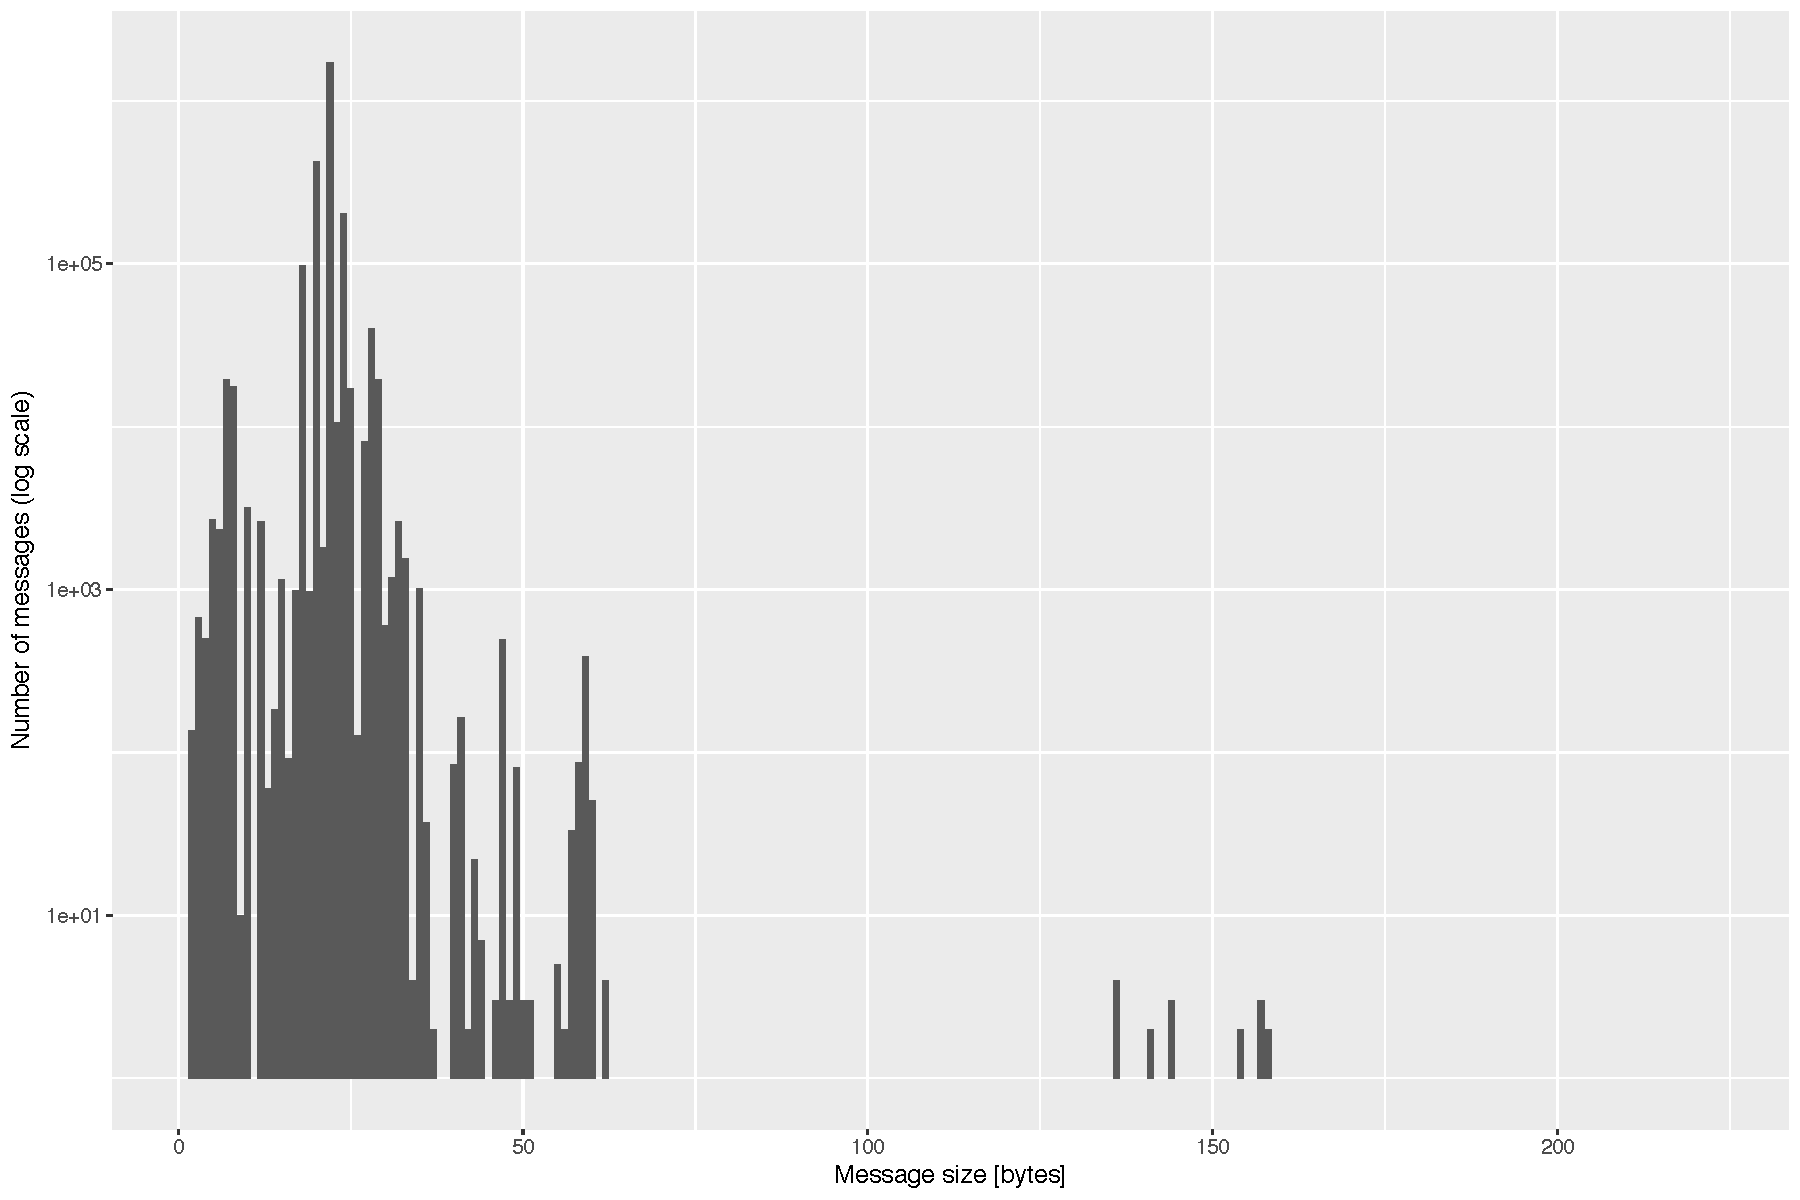
\includegraphics[width=\columnwidth]{figures/sizes.pdf}
  \caption{Message sizes across all gateways (log scale).}
  \label{fig:sizes}
\end{figure}

Figure~\ref{fig:sizes} plots the number of messages received across
all gateways, cumulated by message sizes. Note the logarithmic $y$ axis.
The mode of the distribution is $22$ bytes with a count of over 1.7 million.
A small cluster forms around the value.
Other but distinctly smaller peaks exist. It is difficult to
reason why either exist without knowing more details about the
senders and the applications deployed.
We may remark that the short message size is somewhat congruent
with the prevalent spreading factor seen by the gateways, SF12.
This spreading factor implies more robustness at reception at the
cost of long symbol durations (which in turn make longer messages
more prone to collisions), so messages should be short to achieve
reasonable goodput.
